\chapter{MIRI: The Mid-Infrared Instrument}
MIRI is an instrument that will provide unique capabilities for studying exoplanets and other cold and distant objects. This chapter will provide a detailed overview of the technical details and capabilities of the instrument. A complete description of MIRI is provided in \autocite{MIRI1,MIRI2,10.1086/6822554, MIRI4,MIRI5,MIRI6,MIRI7,MIRI8,MIRI9}
%MIRI is an imaging and spectroscopic instrument on board the James Webb Space Telescope (JWST). 
%
%
\section{The James Webb Space Telescope}
JWST is a 6.5m space based observatory built in collaboration between NASA, ESA and CSA that will be located in a halo orbit at the L2 Earth-Sun Lagrange point. 
As the successor to the Hubble Space Telescope and the Spitzer Space Telescope, it will provide a new perspective for infrared astronomy. 
It is currently scheduled to launch in March 2021.
It will operate at a temperature of 6.7K to reduce instrumental backgrounds over its wavelength range of 0.6-28.8 micron.
A large sun-shield will help maintain the cold operating temperature of the telescope by blocking the solar infrared radiation. 
\begin{figure}[t]
	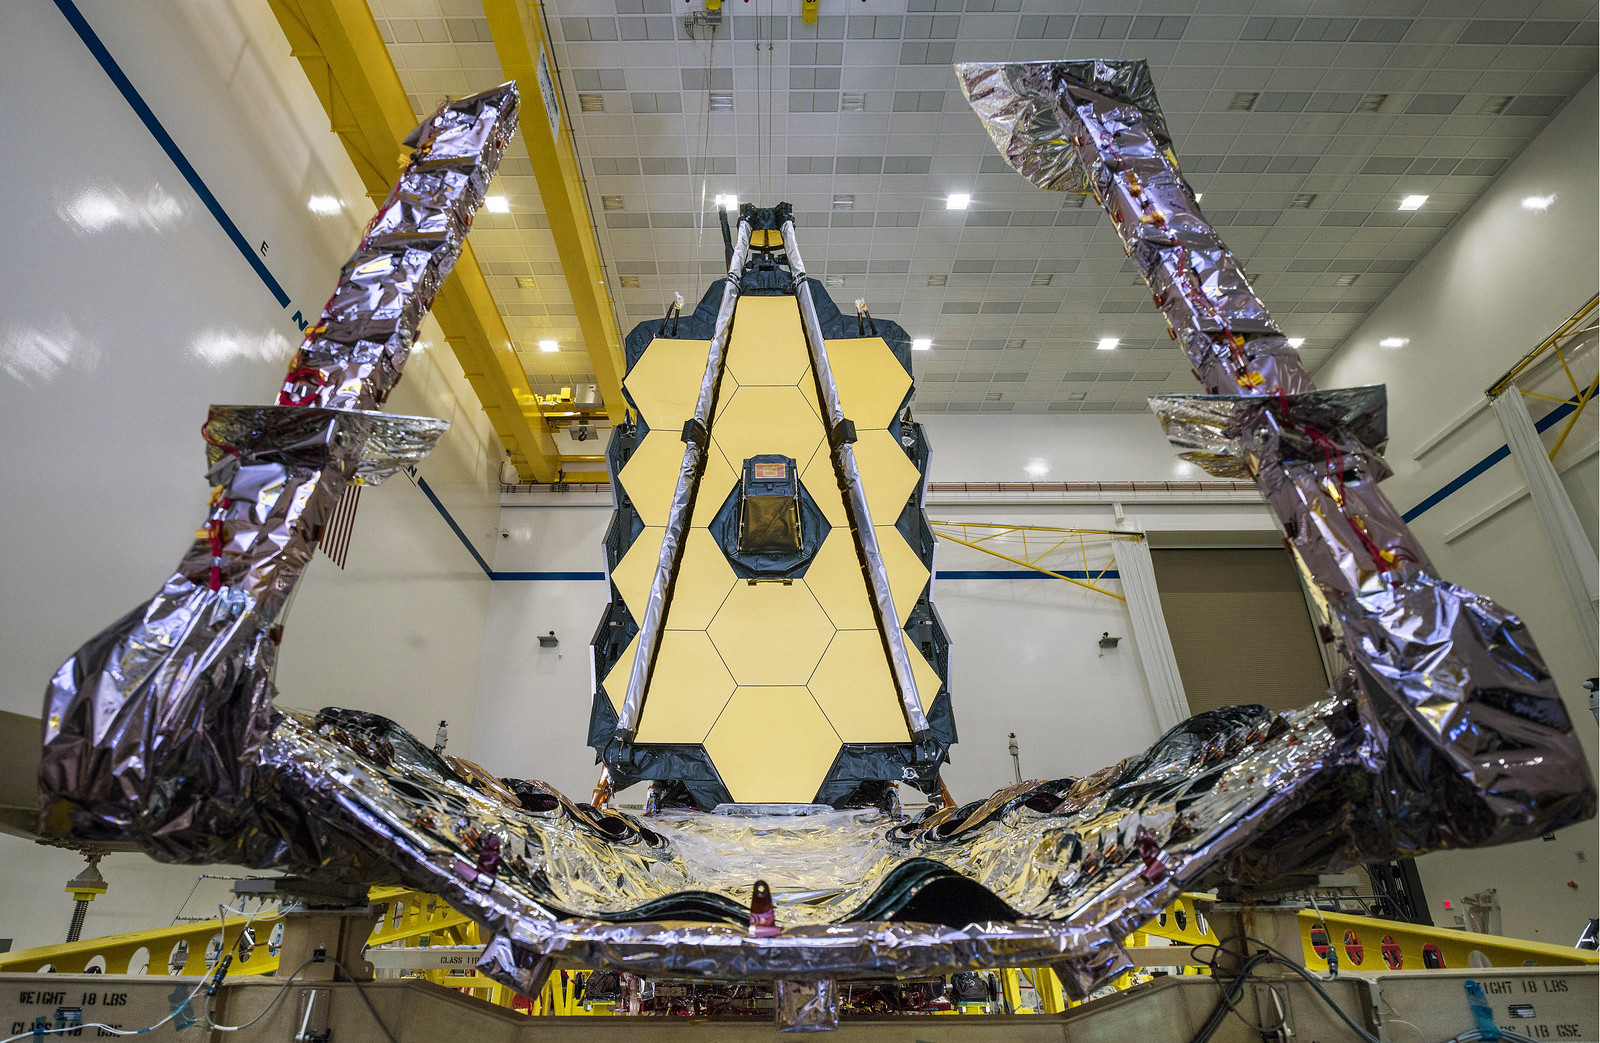
\includegraphics[width=\linewidth]{assembled.jpg}
	\caption{The James Webb Space Telescope during integration of the telescope into the Spacecraft Element \autocite{assembled}. }
	\label{fig:jwst}
\end{figure}

There are four primary instruments that constitute the Integrated Science Instrument Module (ISIM). 
Near-Infrared Camera (NIRCam), which provides imaging with coronagraphic capabilities from 0.6-5 micron.
The Near-Infrared Spectrograph (NIRSpec) provides fixed slit and integrated field unit spectroscopy capable of analyzing multiple objects simultaneously, and operates in the same wavelength range as NIRCam.
The Fine Guidance Sensor/ Near-Infrared Imager and Slitless Spectrograph (FGS/NIRISS) allows for low and medium resolution spectroscopy with high photometric stability, as well as aperture masking interferometry. 
The final instrument, MIRI, is the subject of this thesis.

\section{MIRI}
The Mid-Infrared Instrument (MIRI) provides imaging, fixed slit and integrated field spectroscopy between 4.8 and 28 micron \autocite{Rieke2015}. %MIRI intro

\begin{table}[t]
	\begin{tabular}{l}
		\toprule
		Subsystem\\
		\midrule
		Imaging\\
		4QPM Coronagraphic Imaging\\
		Lyot Coronagraphic Imaging\\
		Low Resolution Spectroscopy\\
		Medium Resolution Spectroscopy\\
		\bottomrule
	\end{tabular}
	\caption{Summary of MIRI observing modes.}
	\label{tab:mirimodes}
\end{table}
\autocite{Kendrew2015} % MIRI IV - LRS
\section{The Medium Resolution Spectrograph}\label{sec:mrs}
The Medium Resolution Spectrograph (MRS) consists of four integrated field spectrographs projected onto two detectors, covering 4.8-28 micron with a spectral resolution varying from R=1700 to R=3500.
\begin{table}[t]
	\centering
	\begin{tabular}{l|lc|cccc}
		\toprule
		Channel & Sub-band & Band & Detector & Wavelength Range [$\mu$m] & FOV [as] & $\lambda$/$\Delta\lambda$\\
		\midrule
		\multirow{3}{*}{1}  &Short & 1A & \multirow{3}{*}{SW}   & 4.83 - 5.82 & 3.46$\times$3.72 & 3500 \\
							&Medium & 1B &						& 5.62 - 6.73 & 3.46$\times$3.72 & 3500 \\
							& Long & 1C&						& 6.46 - 7.76 & 3.41$\times$3.72 & 3300 \\
		\midrule
		\multirow{3}{*}{2}  &Short & 2A & \multirow{3}{*}{SW}   & 7.44 - 8.90 & 4.16$\times$4.76 & 3000 \\
							&Medium & 2B &						& 8.61 - 10.28 & 4.16$\times$4.76 & 3000 \\
							& Long & 2C&						& 9.94 - 11.87 & 4.12$\times$4.76 & 3000 \\
		\midrule
		\multirow{3}{*}{3}  &Short & 3A & \multirow{3}{*}{LW}   & 11.47 - 13.67 & 6.00$\times$6.24 & 2700 \\
							&Medium & 3B &						& 13.25 - 15.80 & 5.96$\times$6.24 & 2300 \\
							& Long & 3C&						& 15.30 - 18.24 & 5.91$\times$6.24 & 2300 \\		
		\midrule
		\multirow{3}{*}{4}  &Short & 3A & \multirow{3}{*}{LW}   & 17.54 - 21.10 & 7.14$\times$7.87 & 1700 \\
							&Medium & 3B &						& 20.44 - 24.72 & 7.06$\times$7.06 & 1700 \\
							& Long & 3C&						& 23.84 - 28.82 & 6.99$\times$7.87 & 1500 \\			
		\bottomrule
	\end{tabular}
	\caption{Properties of the MIRI MRS channels \autocite{MIRI6}.}
	\label{tab:mrs}
\end{table}
\autocite{Wells2015} %MIRI VI MRS
\subsection{Coordinates}
There are three primary coordinate systems in use with JWST/MIRI-MRS, of which two will be relevant for this thesis, with the detector and local MRS coordinates described in Fig. \ref{fig:mrscoords} \autocite{Argyriou2020}.

The detector coordinate grid is formed by counting x/y pixels, as well as the slice number.
Each of the two MRS detectors is an array of 1032$\times$1024 pixels, though only 1024 are photosensitive in the horizontal direction.
Each image slice from the IFU appears as a curved stripe on the detector, though neighboring stripes on the detector do not correspond to neighbouring slices of the image. 

The local MRS coordinate system is described in terms of $\alpha,\beta$ and $\lambda$. The continuous $\alpha$ coordinate is the along slice direction, while $beta$ is perpendicular and discrete, corresponding to the slice number. $\lambda$ is the wavelength. Both $\alpha$ and $\lambda$ are fit by a second order polynomial to account for along and across slice distortion \autocite{MIRI6}. Each detector sub array has its own mapping to $\alpha,\beta,\lambda$ space, due to the differences in FoV, slice count, distortion and spectral resolution.

The third coordinate frame is the global coordinate system of JWST itself, V1,V2,V3. The V1 coordinate refers to the symmetry axis of the telescope, V3 points towards the foldable secondary mirror support structure strut. V2 completes the coordinate system, being orthogonal to V1 and V3. This coordinate system will not be used in this thesis.

\begin{figure}[t]
	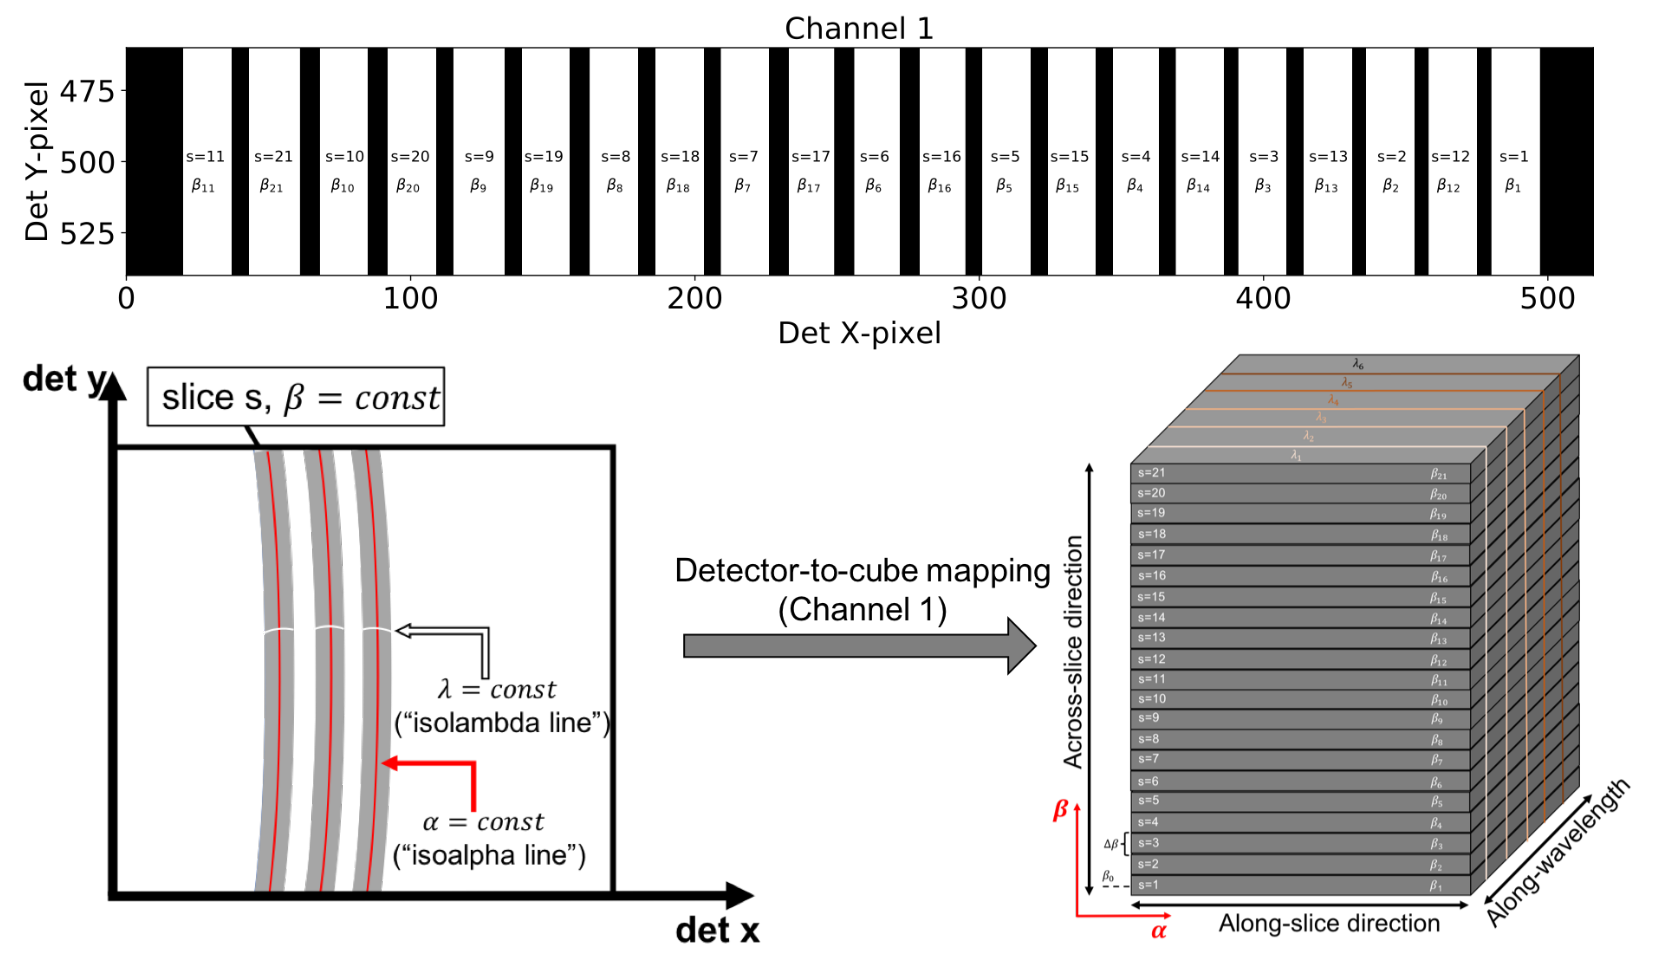
\includegraphics[width=\linewidth]{coordinates.png}
	\caption{Description of the MRS detector (x,y,s) coordinate system to the local MRS ($\alpha,\beta,\lambda$) cube coordinates. \textbf{Top}: Detector coordinates. Note that the consecutive stripe numbers s$_{i}$, s$_{i+1}$ correspond to neighbouring image slices. \textbf{Bottom}: Description of the (invertible) detector-to-cube transformation \autocite{Argyriou2020}.}
	\label{fig:mrscoords}	
\end{figure}

\begin{figure}[t]
	%\includegraphics[width = 0.45\linewidth]{}
	%\includegraphics[width = 0.45\linewidth]{}
	\caption{Detector images of a spatially and spectrally flat calibration source for the SW detector (left) and LW detector (right).}
	\label{fig:flatfield}
\end{figure}
\subsection{Integrated Field Spectroscopy}
\subsection{Optical Systems}
Channels, bands, etc \cite{ref:Chen2019}
\subsection{Detectors}
\subsubsection{Readout Modes}
\section{Observations}
\subsection{Dithering}
\subsection{Exposure time calculations}
